\documentclass{article}

\usepackage[margin=4cm]{geometry}
\usepackage{polyglossia}
	\setmainlanguage{english}
\usepackage{amsmath}
\usepackage{amssymb}
\usepackage{siunitx}
\usepackage{float}
\usepackage{booktabs}
\usepackage{subcaption}
\usepackage{graphicx}
\usepackage{xcolor}
\usepackage{listings}
    \lstset{language=Python,
	basicstyle=\footnotesize\ttfamily,
	breaklines=true,
	framextopmargin=50pt,
	frame=bottomline,
	backgroundcolor=\color{white!85!black},
	commentstyle=\color{blue},
	keywordstyle=\color{red},
	stringstyle=\color{orange!80!black}}
\usepackage{tikz}

\title{Computational Physics - Exercise 9}
\author{Maurice Donner \and Lukas Häffner}

\begin{document}

\maketitle
\newpage

% {{{ Exercise 1
\section{Random Numbers -- Rolling Dice}

We write a simple portable random number generator, using linear congruences:
\begin{align}
    I _{j+1} = a I _{j} + c \ ( \text{mod} \ m )
    \label{LinearCongruence}
\end{align}
For that, we creat an initiation function, that creates a global Variable.

\begin{lstlisting}
def init(initVal):
    global rand
    rand = initVal
\end{lstlisting}

This variable will now be rewritten over and over again by a number generated
by (\ref{LinearCongruence}):

\begin{lstlisting}
def generate_random(a,m,c,initVal):
    global rand
    rand = (a*rand+c)%m
    return rand
\end{lstlisting}

This function produces homogeneously distributed numbers between 0 and m-1.
It can be normalized by \( r_i = I_j /(m-1) \), to get homogeneously distributed
real numbers between 0 and 1. We try it for example for \( a = 106, m = 6075,
c = 1283\):
\begin{lstlisting}
Generating random number... a = 106, m = 6075, c = 1283
Random number sequence:
0: 1389
1: 2717
2: 3760
3: 4968
4: 5441
5: 904
6: 5982
7: 3575
8: 3583
9: 4431

Normalizing...
0: 0.22867961804412248
1: 0.4473164306881791
2: 0.6190319394138953
3: 0.8179124135660191
4: 0.8957853144550544
5: 0.14883108330589398
6: 0.9848534738228515
7: 0.5885742509054989
8: 0.5898913401382944
9: 0.7295027988146197
\end{lstlisting}

A simple way to check 'by eye' that the random number generator really does
produce homogeneously distributed numbers, is to create two sequences with
different initial values \( I_0 \ \text{and} \ J_0 \). 
Let \( \mathbf{r} \) be a random normalized number sequence generated with
\( I_0 = 1 \) and \( \mathbf{s} \) generated with \( J_0 = 2 \).
We plot all pairs \( (r_i, s_i) \) of generated numbers in a number plane:
\begin{figure}[H]
    \centering
    \begin{subfigure}[b]{0.49\linewidth}
	\centering
	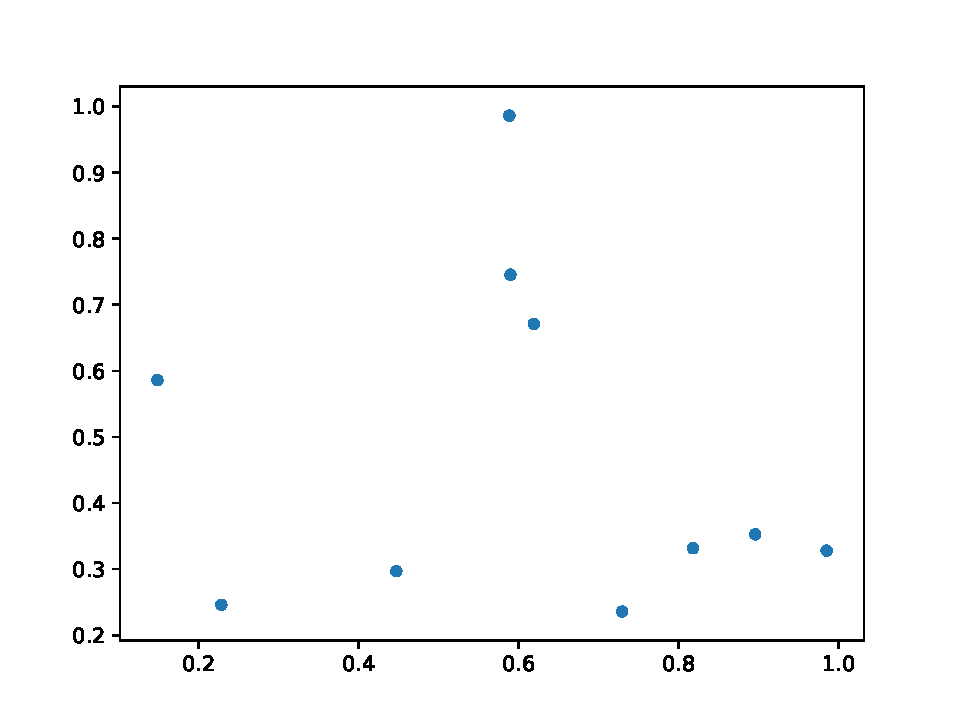
\includegraphics[width=\textwidth]{Fig1-1.pdf} 
	\caption{$n=100$} 
    \end{subfigure}
    \begin{subfigure}[b]{0.49\linewidth}
	\centering
	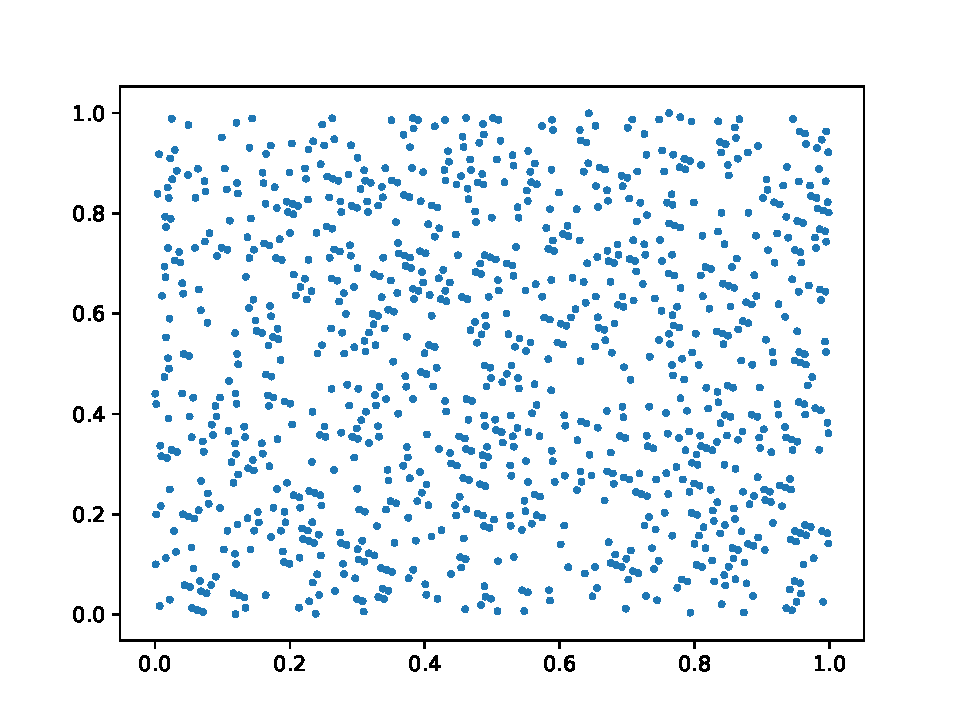
\includegraphics[width=\textwidth]{Fig1-2.pdf} 
	\caption{$n=1000$} 
    \end{subfigure}
    \caption{Creating a set of random numbers}
\end{figure}

Since the eye is quite sensitive to see a good distribution. For \( m = 100\) 
there is no visible pattern. Taking 1000 samples, will result in numbers, that
appear random at first, but this time there are small patterns forming, that
look like little lines all pointing towards the same direction.
To see the deterministic character of this random number sequence, we plot
\( I _{j + 1} \) agains \( I _{j} \) for \( I_0 = 1, \ \text{and} \ n = 1000 \):
\begin{figure}[H]
    \centering
    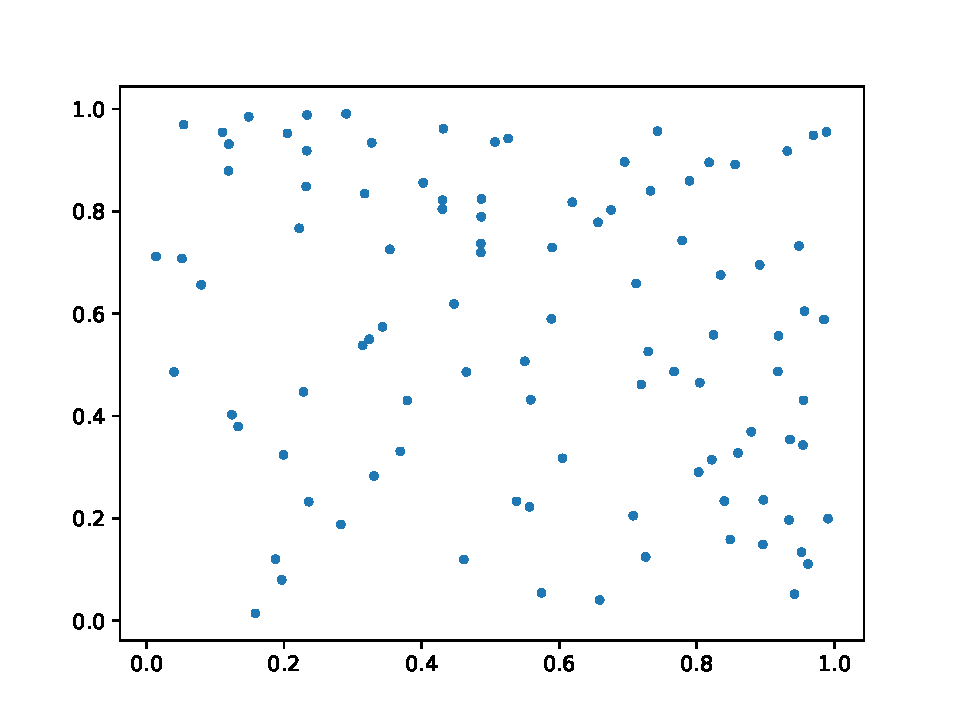
\includegraphics[width=9cm]{Fig1-3.pdf}
    \caption{Deterministic Character of random number sequence}
\end{figure}
Again, overall the generator appears random, yet small patterns can still be seen.
This effect can be midigated, by choosing larger values for a, m, and c.
For example, for \( a = 1060, m = 60751, c = 12835 \), the small patterns,
formerly visible in the deterministic character of our sequence vanishes. (Note,
that choosing prime numbers for \( m \) further counteracts the formation of
patterns)
\begin{figure}[H]
    \centering
    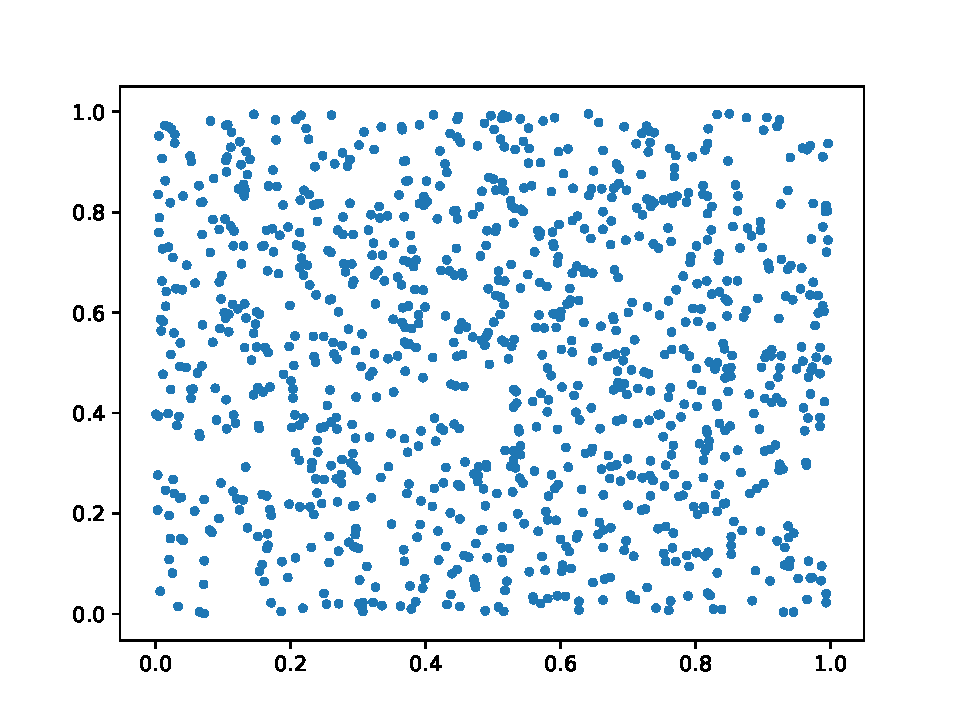
\includegraphics[width=9cm]{Fig1-4.pdf}
    \caption{Choosing larger values $\rightarrow$ The plot becomes "more random"}
\end{figure}

Next we create an experiment where the generator rolls dices. For that, we
normalize our generator to 6, instead of 1 (This will be done in an extra
\texttt{.py} file to avoid confusion). In this configuration, our random number
generator generates numbers between 0 and 6. Because those numbers are equally
distributed, all we need to do is an \texttt{int}-conversion. With that,
python completely neglects any digits behind the comma. And our random numbers
will hence be integer values between 0 and 5. \\
After adding up packets of 10 rolls each, we get a distribution:
\begin{figure}[H]
    \centering
    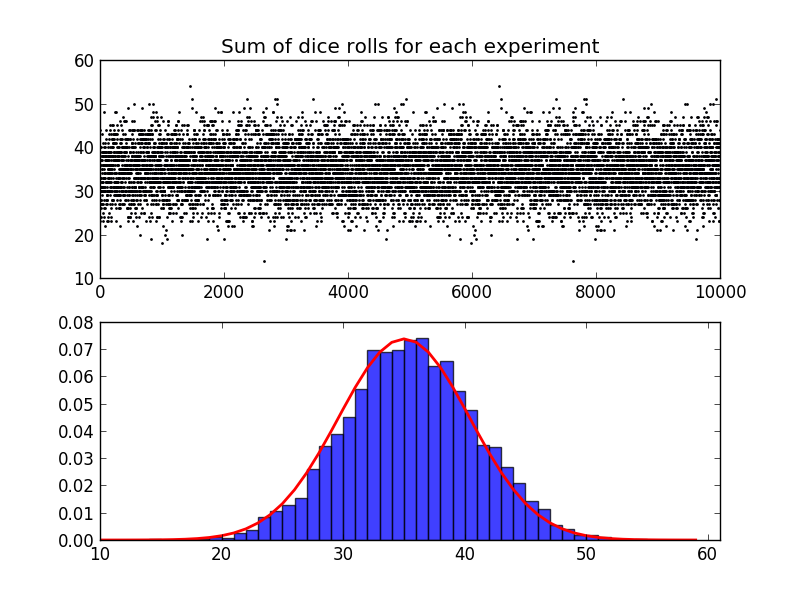
\includegraphics[width=9cm]{Fig1-5.png}
    \caption{Adding 10 Dice rolls -- Distribution}
\end{figure}
The Dice rolls follow a Gaussian Distribution according to the Central Limit
Theorem.
% }}}

% {{{ Exercise 2
\section{Probability distribution functions}

We consider a probablity distribution function given in the domain [0,a) by
\begin{align}
    p(x) = bx \label{2.1}
\end{align}
\begin{figure}[H]
    \centering
    \begin{tikzpicture}
	\draw[->] (0,0) -- (5,0);
	\draw[->] (0,0) -- (0,3.5);
	
	\draw (4, 1pt) -- (4, -1pt) node[anchor=north] {$a$};
	\draw (5,0) node[anchor=north west] {$x$};
	\draw (0,3.5) node[anchor=south east] {$p(x)$};

	\draw[thick, blue!50!black] (0,0) -- (4,3);
	\draw[dashed, blue!50!black] (4,0) -- (4,3.5);
	\draw[dashed, blue!50!black] (0,3) -- (5,3);
    \end{tikzpicture}
    \caption{Probability disribution $p(x)$}
\end{figure}
To norm this distribution, we simply set the value of f(x) at x = a to 1:
\begin{align} \nonumber
    f(a) &\stackrel{!}{=} 1 \\
    &\Rightarrow b \cdot a = 1 \Rightarrow b = \frac{1}{a}
\end{align}
Now we plot again our random number plane, but with the condition, that
\(s_i < f(x_i), \ \text{with} \ x_i = r_i \cdot a\) 
Lastly, we plot a histogram with our generated values, to see if the histogram
indeed follows equation (\ref{2.1}). We experiment with different setsizes:
\begin{figure}[H]
    \centering
    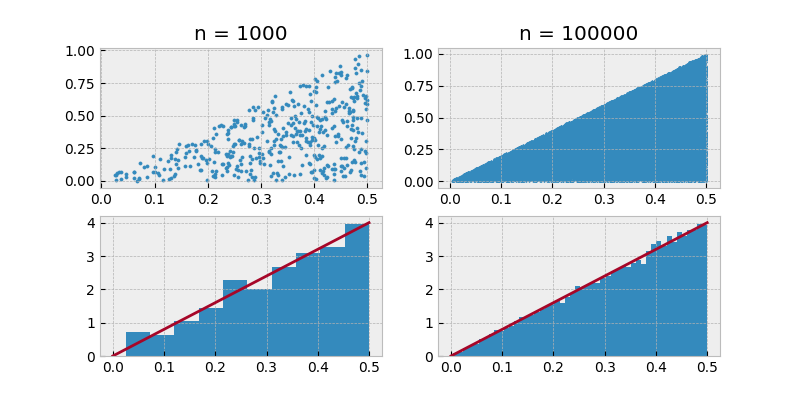
\includegraphics[width=12cm]{Fig2-1.png}
    \caption{Distribution function \( p(x) \)}
\end{figure}
The Histogram has the right shape. However, there seems to be something wrong 
with its normalization. Instead of being normalized to 1, it normalizes to
a value larger than one. \color{red!90!black} This error has not yet been
resolved help please. \color{black}
% }}}

% {{{ Exercise 3
\section{Determine \( \pi \) with random numbers RN}
Lastly we use the same restriction method as before but with the function
\begin{align}
    f(x) = \sqrt{1-x^2} \ \text{for} \ 0 \leq x \leq 1.
\end{align}
Implementing this into code:
\begin{lstlisting}
def rejectionmethod(a,m,c,initVal,steps):
    # initialize with any starting value
    init(initVal)

    # Create Random number distribution
    r_i = ([])
    s_i = ([])
    rej = 0
    acc = 0
    for i in range(steps):
        tmpr = generate_random(a,m,c)/(m-1) # r_i
        tmps = generate_random(a,m,c)/(m-1) # s_i
	f_x = np.sqrt(1-tmpr**2)	    # f(x_i) = b*x_i
        if (tmps < f_x): 
            r_i.append(tmpr)
            s_i.append(tmps)
            acc+=1			    # Count accepted values
        else: 
            rej+=1			    # Count rejected values
    return r_i, s_i, acc, rej
\end{lstlisting}
Using one quadrant of the coordinate system \( (x, f(x) > 0 \), we generate
numbers inside of a quarter of a circle. By dividing the accepted values by
the total number of random numbers, we can estimate the number \( \pi/4 \):
\begin{figure}[H]
    \centering
    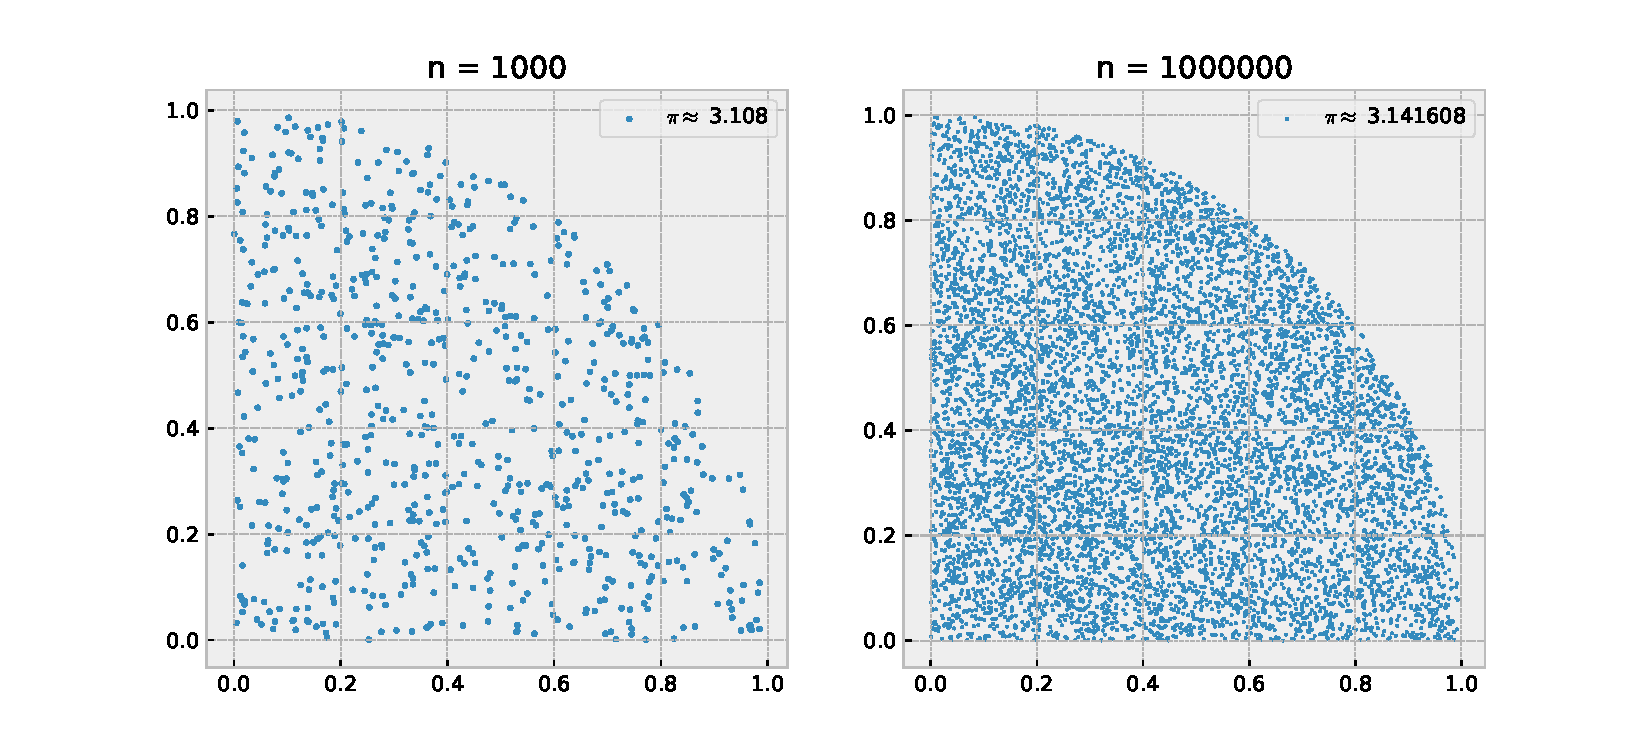
\includegraphics[width=12cm]{Fig3-1.pdf}
    \caption{Approximating \( \pi \) with random numbers}
\end{figure}
Its obvious, that the accuracy of this procedure strongly depends on the amount
of generated numbers, so we rewrite the former code, to iterate through
different stepsizes (for different orders of magnitudes):
\begin{lstlisting}
def rejectionmethod(a,m,c,initVal,N):
    # initialize with any starting value
    init(initVal)

    pi_estimations = np.ndarray((len(N)))
    for setsize in enumerate(N):
        acc = 0
        print(r'Approximating $\pi$ with ', setsize[1], ' random numbers...')
        for i in range(setsize[1]):
            tmpr = generate_random(a,m,c)/(m-1) # r_i
            tmps = generate_random(a,m,c)/(m-1) # s_i
            f_x = np.sqrt(1-tmpr**2)     # f(x_i) = b*x_i
            if (tmps < f_x): 
                acc+=1
        pi_estimations[setsize[0]] = (acc/setsize[1]*4)
    return pi_estimations
\end{lstlisting}
For this function, we choose an array of setsizes \texttt{N} that range between
\( 100 \) and \( 10^n \) with \( n > 2 \) being our desired maximum order of
magnitude. We then plot the Accuracy of our approximated \( \pi \) as a
function of the setsize:
\begin{figure}[H]
    \centering
    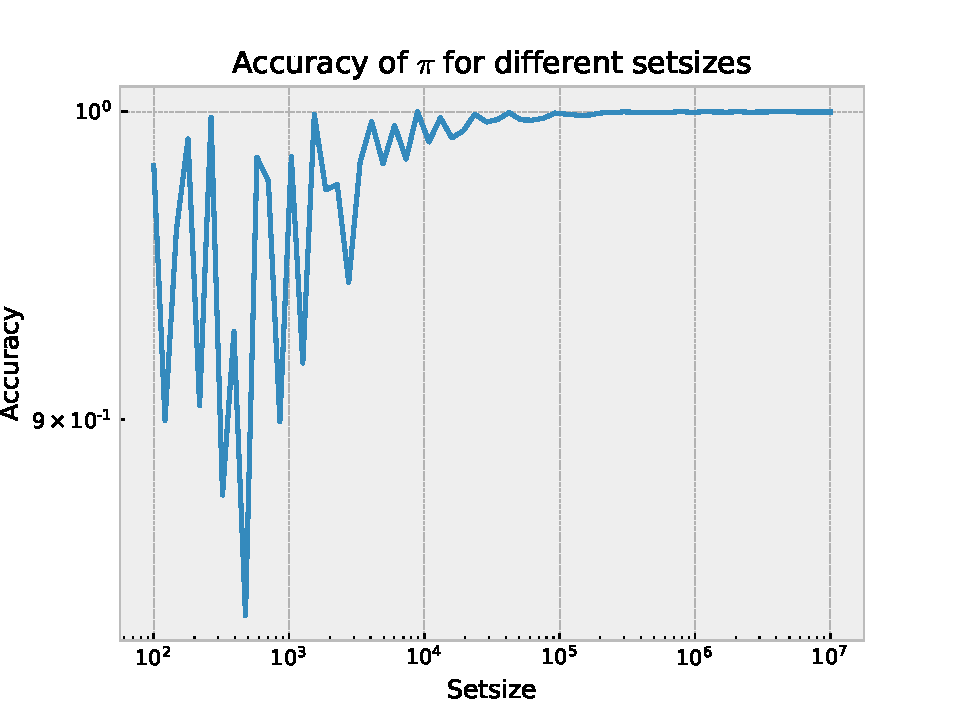
\includegraphics[width=9cm]{Fig3-2.pdf}
    \caption{Accuracy of $pi$ as a function of the setsize $n$}
\end{figure}
Note: This method is not a really good method to approximate \( \pi \) since
our random generator is slightly imperfect. Even for really high values of
\( a, m, \ \text{and} \ c \), tiny patterns emerge and offset the value for
\( \pi \) a little.
% }}}

\end{document}

